\section{Evaluation}
\label{section:evaluation}

Here we present the evaluation of a distributed CQBS broker.
All brokers and coordinators machines were chosen to emulate commodity hardware; for CQBS to be an effective solution, it must not rely on intractably large resources.
Hence, we chose to use the \texttt{t2.medium} AWS instance type with 2 vCPUs and 4 GB RAM, running Ubuntu 14.04.
As we will demonstrate below, the CQBS system is amenable to commodity systems because its performance is limited by the serialization of the etcd log, and not by memory, CPU, disk, or network bandwidth.

\subsection{Broker Performance}

\begin{figure}[t]
\centering
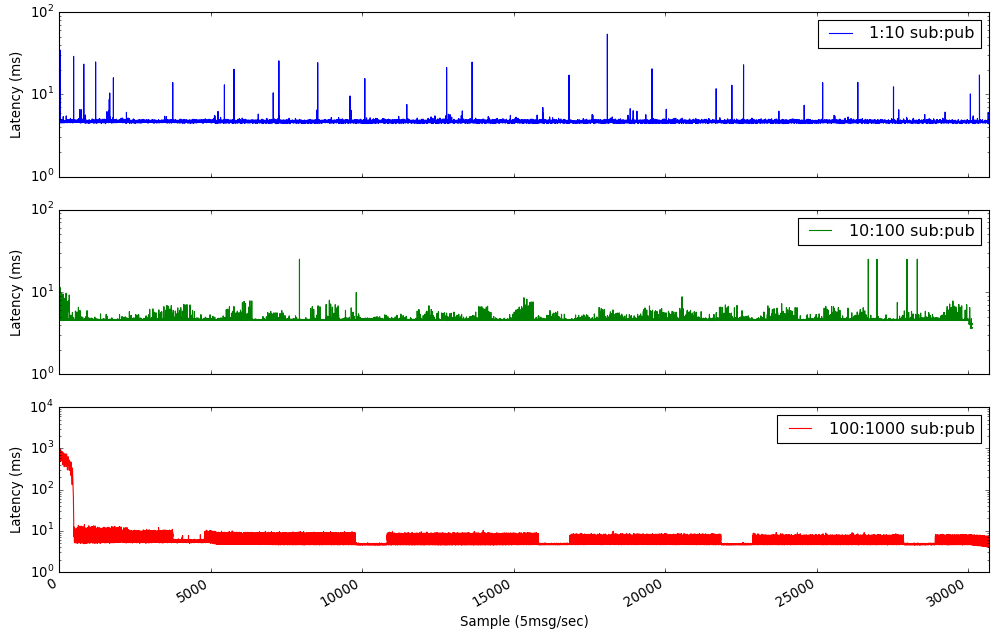
\includegraphics[width=\linewidth]{figs/singlenodelatency.png}
\caption{Microbenchmark: standalone CQBS broker forwarding latency with increasing concurrency}
\label{fig:singlenodelatency}
\end{figure}

First, we examine the latencies of the CQBS broker's forwarding mechanism in isolation---without the communication overhead imposed by the fully replicated system.
We run a single broker on a \texttt{t2.medium} instance, backed by MongoDB\@.
Using a ratio of 10 publishers to one subscriber, we run three benchmarks with 1, 10 and 100 subscribers (with 10, 100 and 1,000 publishers accordingly).
Each publisher sends 5 messages per second; after the initial registration message (the high latencies at the beginning of each benchmark), each publisher sends only its stream UUID and an increasing counter as its value.
Each group of publishers/subscribers use entirely isolated sets of keys, so that they do not explicitly interfere with each other in the broker.
These three microbenchmarks are shown in Figure~\ref{fig:singlenodelatency}, and demonstrate that the latency is fairly consistent as the amount of concurrency scales.

The spikes in latency seen in the $N=1,10$ graphs are due to the pauses enacted by Go's garbage collection.
Fortunately, these do not affect the vast majority of requests.
For the $N=1,10$ cases, the mean latencies, 95\textsuperscript{th} percentile latencies and standard deviation are $4.67ms/4.85ms/0.55ms$ and $4.62ms/4.77ms/0.37ms$ respectively.
For the $N=100$ case, the garbage collection becomes more visible in the variability of response times, with mean, 95\textsuperscript{th} percentile and standard deviation latencies of $13.58ms/8.87ms/67.13ms$.
The troughs in the $N=100$ case are an odd phenomenon, most likely caused by garbage collection in the single Go process used to generate the 100 subscribers and 1000 publishers, generating approximately 5000 messages per second.

\subsection{Coordinator Performance}

\todo{include existing graph}

\subsection{Full-System Performance}

\todo{include existing graph}

\subsection{Fault Tolerance}

\todo{fault tolerance metrics when a broker dies}

\subsection{Client Complexity}

One goal of this system was to maintain a low level of client complexity.
To evaluate this, we have written clients in the Go and Python languages.
Publishers are capable of publishing values and modifying their metadata, and subscribers are capable of submitting queries and attacking handler functions to respond to inbound published messages and notifications about changes to the set of publishers which they are currently subscribed to.
Both types of clients are capable of contacting the coordinator to seamlessly handle the failure of their local broker.

\begin{table}
\centering
\caption{Lines of non-comment, non-whitespace code used to implement programmable clients in Python and Go.
Base Code is the basic code necessary to communicate with the system, Failover is the code necessary to communicate with the coordinator to handle broker failures, and Subscriber/Publisher are the code necessary to implement subscriber- and publisher-specific functionality on top of the shared code.}
\label{tbl:client_code}
\begin{tabular}{ | c | c | c | c | c | c | }
\hline
Language & Base Code & Failover & Subscriber & Publisher & Total
\\\hline
Go & 175 & 111 & 65 & 69 & 420
\\\hline
Python & 105 & 60 & 28 & 33 & 226
\\\hline
\end{tabular}
\end{table}

We present figures for the number of lines of code necessary to create clients in both Go and Python in Table~\ref{tbl:client_code}.
The Python client was easily developed in under one day of effort, indicative of the simple nature of the communication protocol and the ease with which it could be implemented on any number of platforms and devices.
In this regard we consider ourselves highly successful, providing very high availability while managing to require extremely simple client logic.

%%% Local Variables:
%%% mode: latex
%%% TeX-master: "paper"
%%% End:
